\documentclass[../../FisicaTeorica.tex]{subfiles}

\begin{document}

\section{Lezione ?:\\ \large{Titolo}}
\vspace{-1em}
\begin{center}
    \small{(9/11/2018)}
\end{center}

\subsection{Buca finitamente profonda}
\begin{figure}[H]
\centering
\definecolor{qqqqff}{rgb}{0.,0.,1.}
\begin{tikzpicture}[line cap=round,line join=round,>=triangle 45,x=1.0cm,y=1.0cm,scale=0.55]
\draw[->,color=black] (-8.494387027773634,0.) -- (9.293322703354024,0.);
\foreach \x in {-8.,-7.,-6.,-5.,-4.,-3.,-2.,-1.,1.,2.,3.,4.,5.,6.,7.,8.,9.}
\draw[shift={(\x,0)},color=black] (0pt,-2pt);
\draw[->,color=black] (0.,-5.795646939212975) -- (0.,4.380206694230023);
\foreach \y in {-5.,-4.,-3.,-2.,-1.,1.,2.,3.,4.}
\draw[shift={(0,\y)},color=black] (2pt,0pt) -- (-2pt,0pt);
\clip(-8.494387027773634,-5.795646939212975) rectangle (9.293322703354024,4.380206694230023);
\draw [line width=1.2pt,color=qqqqff] (-8.494387027773634,0.)-- (-4.501858550554776,0.);
\draw [dash pattern=on 2pt off 2pt,color=qqqqff] (-4.501858550554776,0.)-- (-4.501858550554776,-4.720199120914791);
\draw [line width=1.2pt,color=qqqqff] (-4.501858550554776,-4.720199120914791)-- (4.501858550554776,-4.720199120914791);
\draw [dash pattern=on 2pt off 2pt,color=qqqqff] (4.501858550554776,-4.720199120914791)-- (4.501858550554776,0.);
\draw [line width=1.2pt,color=qqqqff] (4.501858550554776,0.)-- (9.,0.);
\draw (-5.241319392261099,1.5277626835956077) node[anchor=north west] {$-\frac{a}{2}$};
\draw (4.053159566346146,1.5918625490031226) node[anchor=north west] {$\frac{a}{2}$};
\draw (-7.084190220260811,-3.968800775098799) node[anchor=north west] {$\overline V < 0$};
\draw (-7.949538261234589,1.1431634911505182) node[anchor=north west] {$V = 0$};
\draw (8.31579991632809,-0.186908716055417) node[anchor=north west] {$x$};
\draw (-2.276701103739822,4.2359819970631145) node[anchor=north west] {$V(x)$};
\draw (-8.485438406347642,-1.7573554185395333) node[anchor=north west] {regione 1};
\draw (-3.818323745652703,-3.215627356560498) node[anchor=north west] {regione 2};
\draw (5.543481192467652,-1.8054303175951694) node[anchor=north west] {regione 3};
\begin{scriptsize}
\draw [fill=black] (0.,0.) circle (1.0pt);
\end{scriptsize}
\end{tikzpicture}

\caption{Potenziale della buca finitamente profonda}
\end{figure}

Consideriamo il caso della \textit{buca di potenziale finita}, per cui il potenziale ha la forma $V(x)=\bar{V}\chi_{\left[-\frac{a}{2},\frac{a}{2}\right]}(x)$.\\
Se $\mathcal{E}>0$ la situazione è analoga a quella della barriera di potenziale per $\mathcal{E}>\bar{V}$, solo che qui $\bar{V}<0$ e lì $\bar{V}>0$. In entrambi i casi $\sigma(H)$ è continuo con degenerazione $2$.\\
Anche qui c'è il fenomeno di \textit{risonanza di trasmissione} - una particella \textit{con abbastanza energia} per oltrepassare la barriera ha una probabilità di essere riflessa. In particolare per certe energie la particella \textit{trascorre} più tempo nella regione della buca, e per altri di meno (rispettivamente al tempo calcolato classicamente). Possiamo intuire questo fenomeno se \textit{estendiamo} gli stati discreti presenti nella buca \q{al di sopra} di essa. Quando una particella ha l'energia che \textit{corrisponderebbe} a uno stato discreto \textit{esteso} allora \q{è in risonanza} e trascorre più tempo nella regione della buca.\\

D'altro canto, per $\bar{V}<\mathcal{E}<0$, posti:
\[
\chi=\frac{\sqrt{-2m\mathcal{E}}}{\hbar}; \quad k_2=\frac{\sqrt{2m(\mathcal{E}-\bar{V})}}{\hbar}
\]
Le autofunzioni di $H$ sono:
\[
\varphi_\mathcal{E}(x)=\begin{cases}
c^1_+ e^{\chi x} + c^1_- e^{-\chi x} & x<-\frac{a}{2} \quad (1)\\
c^2_+ e^{ik_2 x} + c^2_- e^{-ik_2 x} & -\frac{a}{2}<x<\frac{a}{2}\quad (2)\\
c^3_+ e^{ik_3 x}+c^3_- e^{-ik_3 x} & x > \frac{a}{2} \quad (3)
\end{cases}
\]
Poiché le autofunzioni (che siano corrispondenti a $\mathcal{E}$ dello spettro discreto o continuo, e quindi siano in\ $\hs$ o $\mathcal{S}'$) non possono divergere esponenzialmente, abbiamo immediatamente che $c^1_- = c^3_+ = 0$.\\

Non serve ora svolgere tutti i conti. Notiamo infatti che, dal caso della barriera con\ $\mathcal{E}<\bar{V}$ otteniamo quello della buca con le sostituzioni:
\begin{align*}
k_1 &\to -i\chi\\
c^3_+ &= 0 =\ c^1_-
\end{align*}
\[
\begin{pmatrix}
c^3_+\\
c^3_-
\end{pmatrix} = (M'M)
\begin{pmatrix}
c^1_+\\
c^1_- = 0
\end{pmatrix}
\]
\[
0 = c^3_+ = (M'M)_{11} \underbrace{c^1_+}_{\neq 0}\Rightarrow (M'M)_{11}=0 
\]
\[
0 = (M'M)_{11} \underset{k_1\to-i\chi}{=}e^{-\chi a}
\left [
\frac{\chi^2-k_2^2-\overbrace{\sin k_2 a}^{(e^{ik_2 a}-e^{-ik_2 a})/(2i)} + \overbrace{\cos(k_2 a)}^{e^{(ik_2 a}+e^-ik_2 a)/2} 2\chi k_2}{2\chi k_2}
\right ]
\]
(*):
\[
(ik_2 + \chi)^2 e^{ik_2 a}=(-ik_2 + \chi)^2 e^{-ik_2 a} \underset{\sqrt{\cdot}}{\Rightarrow} \frac{\chi + ik_2}{\chi-ik_2} = \pm e^{ik_2 a} \Rightarrow c^2_+ = \pm c^2_-
\]
\[
c^2_+ = M_{11}c^1_+; \quad c^2_- = M_{21} c^1_+
\]
\begin{align*}
M_{11} &= \frac{1}{2i}(\chi + ik_2)e^{ik_2 \frac{a}{2}}e^{-\chi\frac{a}{2}}\\
M_{21} &= -\frac{1}{2i}(\chi-ik_2)e^{ik_2 \frac{a}{2}}e^{-\chi\frac{a}{2}}
\end{align*}
\[
\varphi_\mathcal{E}(-x)=\pm \varphi_\mathcal{E}(x)
\]
Prendendo il $+$ otteniamo una funzione pari, e con il $-$ una dispari.\\
Da (*):
\begin{align*}
\op{Re}&\Rightarrow \frac{\chi^2-k_2^2}{\chi^2+k_2^2} = \pm \cos k_2 a\\
\op{Im} &\Rightarrow \frac{2k \chi}{\chi^2 + k_2^2}=\pm \sin k_2 a
\end{align*}

\[
-1+2\left(\frac{\mathcal{E}}{-\bar{V}}\right)=\frac{\chi^2-k_2^2}{\chi^2+k_2^2}=\pm \cos k_2 a = -1+2\begin{cases}
\cos^2\left(k_2\frac{a}{2}\right)\\
\sin^2\left(k_2 \frac{a}{2}\right)
\end{cases}
\]
[TO DO: Correggere segni di $\bar{V}$ in modo che la radici siano ben definite]\\
Soluzione:
\begin{align*}
(1):\>
\begin{cases}
|\cos \frac{k_2 a}{2}| = \sqrt{\frac{\mathcal{E}}{\bar{V}}} = \frac{k_2}{\bar{k}}\\
\sin k_2 a >0
\end{cases} \quad (2):\
\begin{cases}
|\sin \frac{k_2 a}{2} | = \frac{\mathcal{E}}{\bar{V}}\\
\sin \frac{k_2 a}{2} < 0
\end{cases}
\end{align*}
\begin{figure}
\centering
\definecolor{zzttqq}{rgb}{0.6,0.2,0.}
\definecolor{wqwqwq}{rgb}{0.3764705882352941,0.3764705882352941,0.3764705882352941}
\definecolor{ccqqqq}{rgb}{0.8,0.,0.}
\definecolor{ffwwqq}{rgb}{1.,0.4,0.}
\begin{tikzpicture}[line cap=round,line join=round,>=triangle 45,x=1.0cm,y=1.0cm,scale=1.8]
\draw[->,color=black] (-0.3543430138962053,0.) -- (8.074306562308825,0.);
\foreach \x in {,0.5,1.,1.5,2.,2.5,3.,3.5,4.,4.5,5.,5.5,6.,6.5,7.,7.5,8.}
\draw[shift={(\x,0)},color=black] (0pt,-2pt);
\draw[->,color=black] (0.,-0.6826625623217666) -- (0.,2.57489659821151);
\foreach \y in {-0.5,0.5,1.,1.5,2.,2.5}
\draw[shift={(0,\y)},color=black] (2pt,0pt) -- (-2pt,0pt);
\clip(-0.3543430138962053,-0.6826625623217666) rectangle (8.074306562308825,2.57489659821151);
\fill[line width=0.pt,color=zzttqq,fill=zzttqq,fill opacity=0.1] (1.5707963267948966,2.590083354204672) -- (1.5707963267948966,0.) -- (3.1462042425276855,0.) -- (3.1462042425276855,2.590083354204672) -- cycle;
\fill[line width=0.pt,color=zzttqq,fill=zzttqq,fill opacity=0.1] (4.71238898038469,0.) -- (6.2898627331122645,0.) -- (6.2898627331122645,2.590083354204672) -- (4.71238898038469,2.590083354204672) -- cycle;
\draw[line width=1.2pt,color=ffwwqq,smooth,samples=100,domain=-0.3543430138962053:8.074306562308825] plot(\x,{2.0*abs(cos(((\x))*180/pi))});
\draw [color=ccqqqq,domain=-0.3543430138962053:8.074306562308825] plot(\x,{(-0.--1.5118236786901609*\x)/7.633890638507108});
\draw (1.4756610832798418,-0.07519232259528148) node[anchor=north west] {$\frac{\pi}{a}$};
\draw (3.0398969505755504,-0.04481881060895723) node[anchor=north west] {$\frac{2\pi}{a}$};
\draw (4.55097917189519,-0.037225432612376166) node[anchor=north west] {$\frac{3\pi}{a}$};
\draw (6.206335575149872,-0.014445298622632975) node[anchor=north west] {$\frac{4\pi}{a}$};
\draw [dash pattern=on 1pt off 1pt,color=wqwqwq] (1.5707963267948966,0.) -- (1.5707963267948966,2.57489659821151);
\draw [dash pattern=on 1pt off 1pt,color=wqwqwq] (3.1462042425276855,0.) -- (3.1462042425276855,2.57489659821151);
\draw [dash pattern=on 1pt off 1pt,color=wqwqwq] (4.71238898038469,0.) -- (4.71238898038469,2.57489659821151);
\draw [dash pattern=on 1pt off 1pt,color=wqwqwq] (6.2898627331122645,0.) -- (6.2898627331122645,2.57489659821151);
\draw [dash pattern=on 1pt off 1pt,color=wqwqwq,domain=0.0:8.074306562308825] plot(\x,{(--6.292408485055371-2.126671484248277E-5*\x)/3.1462042425276855});
\draw (7.656670772496864,-0.029632054615795104) node[anchor=north west] {$k_2$};
\draw (7.633890638507121,1.5421971906764853) node[anchor=north west] {$\displaystyle\frac{k_2}{\overline k}$};
\draw (0.23794046983712117,2.5976767322012533) node[anchor=north west] {$\left| \cos{\left(\frac{k_2 a}{2}\right)}\right|$};
\draw (1.4932968730918027,2.3774687703004025) node[anchor=north west] {regione proibita};
\draw (4.616581851690057,2.3622820143072403) node[anchor=north west] {regione proibita};
\draw (-0.22525558795432643,2.2939416123380107) node[anchor=north west] {$1$};
\begin{scriptsize}
\draw [fill=black] (0.,0.) circle (1.5pt);
\draw [fill=black] (1.5707963267948966,0.) circle (1.5pt);
\draw [fill=black] (4.71238898038469,0.) circle (1.5pt);
\draw [fill=black] (1.4288359127729424,0.28296815715393125) circle (1.5pt);
\draw [fill=black] (4.27526166628322,0.8466772876040689) circle (1.5pt);
\draw [fill=black] (7.077445924389052,1.4016247860779527) circle (1.5pt);
\draw [fill=black] (3.1462042425276855,0.) circle (1.5pt);
\draw [fill=black] (6.2898627331122645,0.) circle (1.5pt);
\end{scriptsize}
\end{tikzpicture}

\vspace{1cm}

\definecolor{zzttqq}{rgb}{0.6,0.2,0.}
\definecolor{wqwqwq}{rgb}{0.3764705882352941,0.3764705882352941,0.3764705882352941}
\definecolor{ccqqqq}{rgb}{0.8,0.,0.}
\definecolor{ffwwqq}{rgb}{1.,0.4,0.}
\begin{tikzpicture}[line cap=round,line join=round,>=triangle 45,x=1.0cm,y=1.0cm,scale=1.8]
\draw[->,color=black] (-0.3948520356962474,0.) -- (8.379484009221937,0.);
\foreach \x in {,0.5,1.,1.5,2.,2.5,3.,3.5,4.,4.5,5.,5.5,6.,6.5,7.,7.5,8.}
\draw[shift={(\x,0)},color=black] (0pt,-2pt);
\draw[->,color=black] (0.,-0.8150177690400646) -- (0.,2.57614454021208);
\foreach \y in {-0.5,0.5,1.,1.5,2.,2.5}
\draw[shift={(0,\y)},color=black] (2pt,0pt) -- (-2pt,0pt);
\clip(-0.3948520356962474,-0.8150177690400646) rectangle (8.379484009221937,2.57614454021208);
\fill[line width=0.pt,color=zzttqq,fill=zzttqq,fill opacity=0.1] (0.,2.57489659821151) -- (0.,0.) -- (1.566781619238815,0.) -- (1.566781619238815,2.57489659821151) -- cycle;
\fill[line width=0.pt,color=zzttqq,fill=zzttqq,fill opacity=0.1] (3.1462042425276855,2.57489659821151) -- (3.1462042425276855,0.) -- (4.718033487819975,0.) -- (4.718033487819976,2.57489659821151) -- cycle;
\draw[line width=1.2pt,color=ffwwqq,smooth,samples=100,domain=-0.3948520356962474:8.379484009221937] plot(\x,{2.0*abs(sin(((\x))*180/pi))});
\draw [color=ccqqqq,domain=-0.3948520356962474:8.379484009221937] plot(\x,{(-0.--1.5118236786901609*\x)/7.633890638507108});
\draw (1.4785872820025,-0.07196588775870891) node[anchor=north west] {$\frac{\pi}{a}$};
\draw (3.0437391170419597,-0.04034665876801291) node[anchor=north west] {$\frac{2\pi}{a}$};
\draw (4.553557301347701,-0.03244185152033892) node[anchor=north west] {$\frac{3\pi}{a}$};
\draw (6.205662016111575,-0.008727429777316923) node[anchor=north west] {$\frac{4\pi}{a}$};
\draw [dash pattern=on 1pt off 1pt,color=wqwqwq] (3.1462042425276855,0.) -- (3.1462042425276855,2.57614454021208);
\draw [dash pattern=on 1pt off 1pt,color=wqwqwq] (6.2898627331122645,0.) -- (6.2898627331122645,2.57614454021208);
\draw (7.660146549683599,-0.02453704427266492) node[anchor=north west] {$k_2$};
\draw (7.6364321279405765,1.5485195980144606) node[anchor=north west] {$\displaystyle\frac{k_2}{\overline k}$};
\draw (1.7394459211757431,2.599858961955102) node[anchor=north west] {$\left| \sin{\left(\frac{k_2 a}{2}\right)}\right|$};
\draw (-0.06705658035604597,2.3943339735155784) node[anchor=north west] {regione proibita};
\draw (3.053645828691943,2.354809937277208) node[anchor=north west] {regione proibita};
\draw (-0.22094627624741847,2.291571479295816) node[anchor=north west] {$1$};
\draw [dash pattern=on 1pt off 1pt,color=wqwqwq] (1.566781619238815,0.) -- (1.566781619238815,2.57614454021208);
\draw [dash pattern=on 1pt off 1pt,color=wqwqwq] (4.718033487819975,0.) -- (4.718033487819975,2.57614454021208);
\draw [dash pattern=on 1pt off 1pt,color=wqwqwq,domain=0.0:8.379484009221937] plot(\x,{(--3.133537985318499-0.*\x)/1.566781619238815});
\draw (6.204425462532493,2.3785243590202305) node[anchor=north west] {(regione proibita...)};
\begin{scriptsize}
\draw [fill=black] (0.,0.) circle (1.5pt);
\draw [fill=black] (8.436027293701917,1.670679660035962) circle (1.5pt);
\draw [fill=black] (3.1462042425276855,0.) circle (1.5pt);
\draw [fill=black] (6.2898627331122645,0.) circle (1.5pt);
\draw [fill=black] (2.8549829065558936,0.5654037976949899) circle (1.5pt);
\draw [fill=black] (5.685229235738035,1.1259087361975673) circle (1.5pt);
\draw [fill=black] (1.566781619238815,0.) circle (1.5pt);
\draw [fill=black] (4.718033487819975,0.) circle (1.5pt);
\end{scriptsize}
\end{tikzpicture}
\caption{(1) e (2) in funzione di $k_2$, plot di membro sx, dx e intersezioni (soluzioni)}
\end{figure}
\[
\bar{k}=\frac{\sqrt{-2m\bar{V}}}{\hbar}
\]
Le soluzioni a (1) e (2) sono le soluzioni dell'equazioen agli autovalori per $H$ con $\mathcal{E}<0$. Notiamo che è unicamente discreto, e quindi le autofunzioni $\varphi_\mathcal{E}(x)\in L^2$. 
\[
\sigma(H)\Big|_{\mathcal{E}<0}=\sigma_P(H) \text{ e non degenere (degenerazione $1$)}
\]
Se $\bar{V}\to\infty$ la retta $k_2/\bar{k}$ tende all'asse $x$ ed esaminandone le intersezioni con $\cos$ e $\sin$ ritroviamo i risultati della buca infinitamente profonda.\\

\subsection{Regole generali per $\sigma(H)$ per potenziali in $1D$ (con al più salti)}
\begin{figure}[H]
\centering
\definecolor{qqqqff}{rgb}{0.,0.,1.}
\begin{tikzpicture}[line cap=round,line join=round,>=triangle 45,x=1.0cm,y=1.0cm]
\draw[->,color=black] (-6.676479077874541,0.) -- (8.002026159205059,0.);
\foreach \x in {-6.,-5.,-4.,-3.,-2.,-1.,1.,2.,3.,4.,5.,6.,7.,8.}
\draw[shift={(\x,0)},color=black] (0pt,-2pt);
\draw[->,color=black] (0.,-1.67819159971909) -- (0.,3.569434852014872);
\foreach \y in {-1.,1.,2.,3.}
\draw[shift={(0,\y)},color=black] (2pt,0pt) -- (-2pt,0pt);
\clip(-6.676479077874541,-1.67819159971909) rectangle (8.002026159205059,3.569434852014872);
\draw [shift={(-5.990479550422295,-0.503060335720243)},line width=1.2pt,color=qqqqff]  plot[domain=0.921463135200873:1.5745998322606323,variable=\t]({1.*2.503078441283073*cos(\t r)+0.*2.503078441283073*sin(\t r)},{0.*2.503078441283073*cos(\t r)+1.*2.503078441283073*sin(\t r)});
\draw [shift={(-4.087433525065524,1.9823996714100185)},line width=1.2pt,color=qqqqff]  plot[domain=4.042484887064738:5.68560406525681,variable=\t]({1.*0.6273784139167422*cos(\t r)+0.*0.6273784139167422*sin(\t r)},{0.*0.6273784139167422*cos(\t r)+1.*0.6273784139167422*sin(\t r)});
\draw [shift={(-3.4056119847292083,1.5137154376894562)},line width=1.2pt,color=qqqqff]  plot[domain=0.5137956939737662:2.524824404105156,variable=\t]({1.*0.20002216638462805*cos(\t r)+0.*0.20002216638462805*sin(\t r)},{0.*0.20002216638462805*cos(\t r)+1.*0.20002216638462805*sin(\t r)});
\draw [shift={(-2.9526513154048626,1.782574813850848)},line width=1.2pt,color=qqqqff]  plot[domain=3.6906518165667066:5.6252594582745346,variable=\t]({1.*0.32679849406407757*cos(\t r)+0.*0.32679849406407757*sin(\t r)},{0.*0.32679849406407757*cos(\t r)+1.*0.32679849406407757*sin(\t r)});
\draw [shift={(-0.9591334354802966,0.12882822270892555)},line width=1.2pt,color=qqqqff]  plot[domain=1.6195474014402678:2.4440924849192416,variable=\t]({1.*2.263597170879376*cos(\t r)+0.*2.263597170879376*sin(\t r)},{0.*2.263597170879376*cos(\t r)+1.*2.263597170879376*sin(\t r)});
\draw [shift={(-1.0778080450689216,1.4151124162679072)},line width=1.2pt,color=qqqqff]  plot[domain=0.3193308056715693:1.5622132016919401,variable=\t]({1.*0.9746595027453426*cos(\t r)+0.*0.9746595027453426*sin(\t r)},{0.*0.9746595027453426*cos(\t r)+1.*0.9746595027453426*sin(\t r)});
\draw [shift={(-39.042773991560445,-14.365568665496033)},line width=1.2pt,color=qqqqff]  plot[domain=0.3360384106053099:0.3922105553849662,variable=\t]({1.*42.08610264399796*cos(\t r)+0.*42.08610264399796*sin(\t r)},{0.*42.08610264399796*cos(\t r)+1.*42.08610264399796*sin(\t r)});
\draw [shift={(1.165296596585405,-0.3180909616447532)},line width=1.2pt,color=qqqqff]  plot[domain=3.4839282860822745:5.834909745929153,variable=\t]({1.*0.5052276175177605*cos(\t r)+0.*0.5052276175177605*sin(\t r)},{0.*0.5052276175177605*cos(\t r)+1.*0.5052276175177605*sin(\t r)});
\draw [shift={(3.2013198737488575,1.237545130990266)},line width=1.2pt,color=qqqqff]  plot[domain=0.5404927744988528:2.7834973068748012,variable=\t]({1.*0.7488204882226647*cos(\t r)+0.*0.7488204882226647*sin(\t r)},{0.*0.7488204882226647*cos(\t r)+1.*0.7488204882226647*sin(\t r)});
\draw [shift={(5.964690534938655,2.98677397119538)},line width=1.2pt,color=qqqqff]  plot[domain=3.713006848920577:4.202967265019543,variable=\t]({1.*2.5219323972745222*cos(\t r)+0.*2.5219323972745222*sin(\t r)},{0.*2.5219323972745222*cos(\t r)+1.*2.5219323972745222*sin(\t r)});
\draw [shift={(7.273630176071871,5.41887749611166)},line width=1.2pt,color=qqqqff]  plot[domain=4.211168131805285:4.690363138666036,variable=\t]({1.*5.283735136003091*cos(\t r)+0.*5.283735136003091*sin(\t r)},{0.*5.283735136003091*cos(\t r)+1.*5.283735136003091*sin(\t r)});
\draw [line width=1.2pt,color=qqqqff] (7.157260872005046,0.13642397785855528)-- (8.109235623814909,0.13642397785855528);
\draw [line width=1.2pt,color=qqqqff] (-6.,2.)-- (-6.7208191960118535,2.);
\draw (-1.2679573336892247,3.408540644768312) node[anchor=north west] {$V(x)$};
\draw (5.1554357675285765,1.3911748154460577) node[anchor=north west] {$V(x \to \infty) = 0 $};
\draw (7.234684401448789,-0.18063782457803) node[anchor=north west] {$x$};
\draw (0.8731737000500424,-0.9851088608108308) node[anchor=north west] {$V_\text{min}$};
\draw (-6.552714278236433,2.7649638157820715) node[anchor=north west] {$V(x \to -\infty) > 0$};
\draw [shift={(-32.53547830222711,15.417631168735921)},line width=1.2pt,color=qqqqff]  plot[domain=5.8460770521613865:5.9050571062125305,variable=\t]({1.*37.69861001701251*cos(\t r)+0.*37.69861001701251*sin(\t r)},{0.*37.69861001701251*cos(\t r)+1.*37.69861001701251*sin(\t r)});
\begin{scriptsize}
\draw [fill=qqqqff] (1.1610008339262132,-0.8233003161957635) circle (1.5pt);
\end{scriptsize}
\end{tikzpicture}
\caption{Potenziale $V(x)$ generico}
\end{figure}

Consideriamo un potenziale generico $V(x)$, con $V(x\to + \infty)=0$, con al più discontinuità di salto, e $V(x\to-\infty) > 0$.\\
Si hanno tre possibili situazioni qualitative:
\begin{enumerate}
\item $\min V(x) < \mathcal{E} < 0$. Allora per $x\to \pm \infty$, $\varphi_\mathcal{E}\sim e^{\mp c_\pm x}$ (non può divergere, e in particolare $\varphi_\mathcal{E}\in \hs$).\\
Lo spettro è non degenere (deg. 1) perché se $\psi_1$ e $\psi_2$ sono soluzioni corrispondenti alla stessa energia $\mathcal{E}$:
\begin{align*}
\psi_1'' + \frac{2m}{\hbar^2}(\mathcal{E}-V(x))\psi_1 &= 0\\
\psi_2'' + \frac{2m}{\hbar^2}(\mathcal{E}-V(x))\psi_2 &= 0
\end{align*}
Dividendo la prima per $\psi_1$ e la seconda per $\psi_2$ si ha:

\begin{align*}
\frac{\psi_1''}{\psi_1}=\frac{2m}{\hbar^2}((V(x)-\mathcal{E})=\frac{\psi_2''}{\psi_2} &\Rightarrow \psi_1''\psi_2 - \psi_1\psi_2'' = 0\\
&= \frac{d}{dx}(\psi_1' \psi_2 - \psi_1 \psi_2') = 0
\end{align*}
E quindi $(\psi_1'\psi_2 - \psi_1 \psi_2')$ deve essere costante.\\
Per regolarità $\mathcal{E}\in \sigma_P(H) \Rightarrow  \exists \psi_{1/2}(\pm\infty)$ e quindi deve essere $0$ (essendo in $\hs$). Ma allora:
\[
(\psi_1' \psi_2 - \psi_1 \psi_2')(x=\infty)=0\Rightarrow \ln \psi_1 = \ln \psi_2 + \text{cost} \Rightarrow \psi_1(x)=\psi_2(x)e^{?\text{cost}}
\]
e quindi $\psi_1$ e $\psi_2$ differiscono per un fattore moltplicativo, ossia definiscono lo \textbf{stesso stato}.\\
Perciò:
\[
\sigma(H)\Big|_{V_{min} < \mathcal{E} < 0} \text{ non degenere }
\]
\item Se invece $0 < \mathcal{E} < V(-\infty)$ la soluzione ha l'andamento:
\[
\varphi_\mathcal{E}(x) = \begin{cases}
c_+ e^{ikx} + c_-e^{-ikx} & x\to\infty\\
e^{\chi x} & x\to-\infty
\end{cases} \quad \chi =\ \frac{\sqrt{2m(V(+\infty)-\mathcal{E})}}{\hbar}
\]
Poiché la soluzione oscilla infinitamente $\notin \hs$, e quindi lo spettro di $H$ è continuo:
\[
\sigma(H)\Big|_{0<\mathcal{E}<V(-\infty)} \text{ è continuo }
\]
Perché $\varphi_\mathcal{E}(-\infty) = 0$ possiamo applicare gli stessi ragionamenti del teorema visto al punto precedente e quindi affermare che la degenerazione di $\sigma(H)$ è $1$ (non degenerato).
\item Nel caso $\mathcal{E} > V(-\infty)$ ($> V(+\infty)$). Le soluzioni:
\[
\varphi_\mathcal{E}(x) = \begin{cases}
c^1_+ e^{ikx} + c^1_- e^{-ikx} & x\to +\infty\\
c^2_+ e^{ik_1 x} + c^2_- e^{-ik_1 x} & x\to -\infty
\end{cases}
\]
con
\[
k_1 =\ \frac{\sqrt{2m(\mathcal{E}-V(-\infty))}}{\hbar}
\]
Anche in questo caso le autofunzioni non sono in $\hs$ (presentano oscillazioni infinite) e allora:
\[
\sigma(H)\Big|_{\mathcal{E}>V(-\infty)} \text{ è continuo con deg. 2}
\]
(degenerazione: $4$ costanti da determinare - $2$ condizioni di raccordo $= 2$).
\end{enumerate}
Se definiamo la parità $\mathcal{P}$:
\[
(\mathcal{P}\psi)(x)=\psi(-x)
\]
Se $V(x)=V(-x)$ allora se $\varphi_\mathcal{E}(x)$ è soluzione dell'equazione di Schrodinger stazionaria,a nche $\varphi_\mathcal{E}(-x)$ lo è, e se lo spettro $\sigma(H)$ è non degenere deve essere $\varphi_\mathcal{E}(x)=c \varphi_\mathcal{E}(-x) = c^2\varphi_\mathcal{E}(x)$, e quindi $c=\pm 1$.\\
Vi sono solo due possibilità: o $\varphi_\mathcal{E}(x) =\varphi_\mathcal{E}(-x)$ pari, oppure $\varphi_\mathcal{E}(x)=-\varphi_\mathcal{E}(-x)$ dispari.\\
Perciò in tal caso gli autostati di $H$ sono anche autostati della parità $\mathcal{P}$.

\subsection{Esercizio}
Una particella di massa $m$ si trova nello stato fondamentale (cioè di energia minima) in una buca di potenziale infinita in $[0,a]$. Al tempo $t = 0$ la parete impenentrabile posta in $a$ viene improvvisamente spostata in $x=2a$. \begin{enumerate}
\item Calcolare la probabilità che al tempo $\bar{t}>0$ l'energia della particella sia uguale a quella a $t=0^-$
\item Che sia invece minore.
\end{enumerate}
%[PLOT] della funzione d'onda a t=0^- e t=0^+
\begin{figure}[H]
\centering
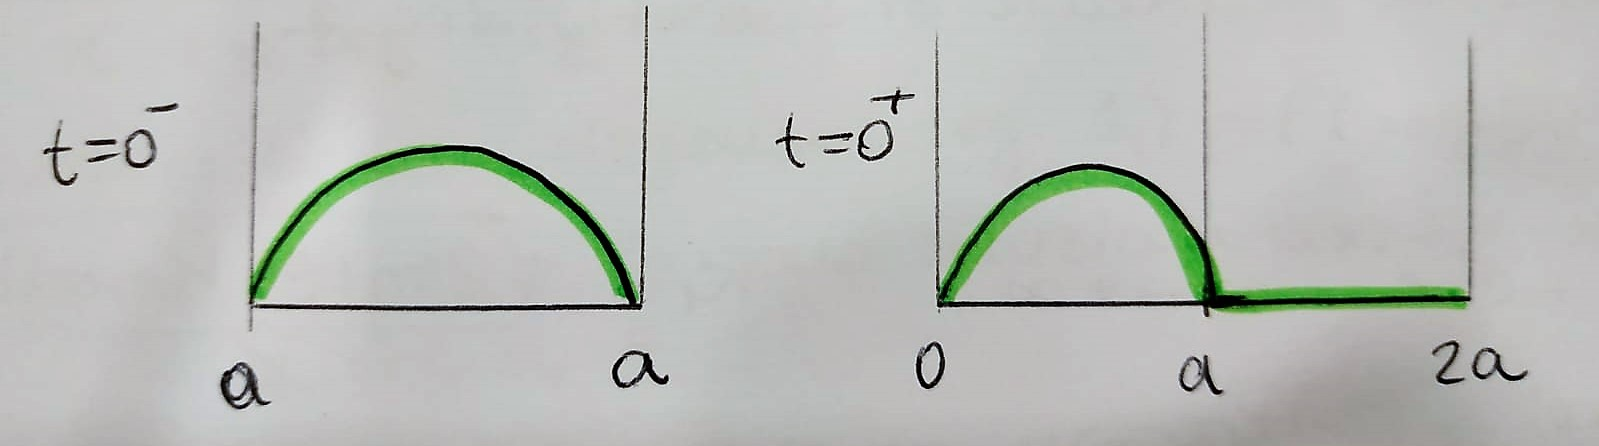
\includegraphics[scale=0.3]{Immagini/Im5.jpeg}
\caption{Funzione d'onda $\psi$ per $t=0^-$ e $t=0^+$}
\end{figure}
\begin{itemize}
\item Per $t<0$, $\sigma(H_1)$ è quello della buca in $[0,a]$, e gli autovalori sono:
\[
\mathcal{E}^1_n = \frac{\hbar^2}{2m}\frac{\pi^2 n^2}{a^2}
\]
\item Per $t>0$, la buca è in $[0,2a]$ e gli autovalori saranno:
\[
\mathcal{E}^2_n = \frac{\hbar^2}{2m}\frac{\pi^2 m^2}{4a^2}
\]
\end{itemize}
Dopo il cambiamento del sistema, la $\psi$ non è più autofunzione di $H$. Confrontando le due espressioni per gli autovalori, si ha che:
\[
\mathcal{E}^1_1 = \mathcal{E}^2_2
\]
Quindi per rispondere alla prima richiesta occorre calcolare $W_{\psi(t>0)}^{H_2} (\mathcal{E}_2^2)$, ossia la probabilità che una misura di energia a $t>0$ dia come risultato $\mathcal{E}_2^2$.\\
In notazione di Dirac:
\begin{align*}
W_{\psi(t)}^{H_2}(\mathcal{E}_2^2)&=|\braket{\psi(t)|\mathcal{E}_2^2}|^2 = |\bra{\psi(0^+)}e^{i\frac{t}{\hbar}H_2}\ket{\mathcal{E}_2^2}|^2 = \\
&=|\braket{\psi(0^+)|\mathcal{E}^2_2} e^{i\frac{t}{\hbar}\mathcal{E}_2^2}|^2 = |\braket{\psi(0^+)|\mathcal{E}_2^2}|^2
\end{align*}
dove abbiamo semplificato l'evoluzione temporale riducendola al calcolo della $\psi$ in $t=0^+$.\\
Abbiamo quindi:
\[
\psi(x,t=0^-) = \begin{cases}
\sqrt{\frac{2}{a}} \sin \frac{\pi}{a}x & x \in [0,a]\\
0 & \text{altrove}
\end{cases}
\]
\[
\psi(x,t=0^+) = \begin{cases}
\psi(x,t=0^-) & x \in [0,a]\\
0 & \text{altrove}
\end{cases}
\]
ed è già normalizzata in $L^2([0,2a],dx)$ (era normalizzata prima, e abbiamo aggiunto solo degli zeri).\\
Calcoliamo l'autofunzione di $H_2$:
\[
\braket{x|\mathcal{E}_n^2}=\varphi_n(x)=\sqrt{\frac{1}{a}} \sin \frac{\pi x n}{2a}
\]
Se vogliamo quindi calcolare il prodotto scalare (per esprimere la $\psi$ sulla base delle autofunzioni di $H_2$):
\begin{align*}
\braket{\psi(0^+)|\mathcal{E}_2^2} &= \int_0^a \sqrt{\frac{2}{a}}\sin \frac{\pi x}{a} \sqrt{\frac{2}{a}}\sin \frac{2\pi x}{2a} dx +\int_a^{2a} 0\cdot \sqrt{\frac{1}{a}} \sin \frac{2\pi x}{2a}dx =\\
&= \frac{\sqrt{2}}{a}\int_0^a \sin^2 \frac{\pi x}{a}= \frac{\sqrt{2}}{a}\frac{a}{2}=\frac{1}{\sqrt{2}}
\end{align*}
E allora:
\[
W^{H_2}_{\psi(t>0)}(\mathcal{E}_2) = \frac{1}{2}
\]
Per rispondere alla domanda $2$, dato che l'unico autovalore di $H_2$ con energia minore di $\mathcal{E}_2^2=\mathcal{E}_1^1$ è quello per $n=1$, basta calcolare $W^{H_2}_{\psi(t)}(\mathcal{E}_1^2)$.\\
Utilizzando la notazione di Dirac:
\[
W^{H_2}_{\psi(t)}(\mathcal{E}_1^2) = |\braket{\psi(0^+)|\mathcal{E}_1^2}|^2
\]
Calcolando:

\begin{align*}
\braket{\psi(0^+)|\mathcal{E}_1^2} &= \int_0^a \sqrt{\frac{2}{a}} \sin \frac{\pi x}{a} \sqrt{\frac{1}{a}} \sin \frac{\pi x}{2a} dx\underset{(a)}{=} \frac{\sqrt{2}}{a} \int_0^a \frac{1}{2} \left [
\cos \frac{\pi a}{2a}-\cos \frac{3\pi x}{2a}
\right ]dx =\\
&\underset{(b)}{=}\frac{\sqrt{2}}{a}\frac{1}{2}\left [
\frac{2a}{\pi} \sin y \Big |_0^{\frac{\pi}{2}} - \frac{2a}{3\pi}\sin y \Big|_{0}^{\frac{3}{2}\pi}\right ] = \sqrt{2}\left [
\frac{1}{\pi}+\frac{1}{3\pi}
\right] = \sqrt{2}\frac{4}{3\pi}
\end{align*}
dove in (a) si è usata la formula di prostaferesi:
\[
\sin \alpha \sin \beta= \frac{1}{2}[\cos(\alpha-\beta)-\cos(\alpha+\beta)]
\]
e in (b) si è effettuato il cambio di variabili $y=\pi x/(2a)$.
Arriviamo quindi:
\[
W_{\psi(t)}^{H_2}(\mathcal{E}_1^2)=\frac{32}{9\pi^2}
\]
\end{document}